\section{Clustering}

\begin{frame}
    \frametitle{Clustering}
    \begin{exampleblock}{Preparation }
        
    
        \begin{itemize}
            \item IQR method for outliers detection
            \item Min-Max scaling
            \item Silhouette score for evaluation
        \end{itemize}
    \end{exampleblock}    
\end{frame}

%%%%%%%%%%%%%%%%%%%%%%%%%%%%%%%%%%%%%%%%%%%%%%%%%%%%%%%%%%%%%%%%%%%%%%%%%%

\begin{frame}
    \frametitle{Clustering}

\begin{exampleblock}{K-Means}
    \begin{itemize}
        \item Entire dataset
        \item Parameter: $k$ (number of clusters)
    \end{itemize}
\end{exampleblock}
\begin{exampleblock}{DBSCAN}
    \begin{itemize}
        \item State: California
        \item Parameters: {
            \begin{itemize}
                \item $\epsilon$ (neighborhood radius)
                \item $n$ (core points neighborhood minimum size)
            \end{itemize}
        }
        
    \end{itemize}
\end{exampleblock}
\begin{exampleblock}{Hierarchical}
    \begin{itemize}
        \item State: California
        \item Parameter: inter-cluster distance
    \end{itemize}
\end{exampleblock}

\end{frame}

%%%%%%%%%%%%%%%%%%%%%%%%%%%%%%%%%%%%%%%%%%%%%%%%%%%%%%%%%%%%%%%%%%%%%%%%%%

\begin{frame}{K-means}
    \begin{exampleblock}{Selected features:}
        \begin{itemize}
            \item state\_population
            \item timestamp
            \item p\_injured
            \item month\_cd\_change\_min\_age\_participants
            \item month\_cd\_ratio\_males
        \end{itemize}        
    \end{exampleblock}


    
    \begin{table}[]
        \centering
        \begin{tabular}{|lc|}
    
            \hline
            \textbf{Clustering}  & C6 \\
            \textbf{K} & 2\\
            \textbf{Clusters sizes} & (59466, 35725) \\
            \textbf{Silhouette mean} & 0.453778 \\
            \textbf{Silhouette variance} & 3.048582e-08 \\
            \hline

        \end{tabular}
        \label{tab:my_label}
    \end{table}
\end{frame}

%%%%%%%%%%%%%%%%%%%%%%%%%%%%%%%%%%%%%%%%%%%%%%%%%%%%%%%%%%%%%%%%%%%%%%%%%%

\begin{frame}{K-means}
    \begin{figure}
        \centering
        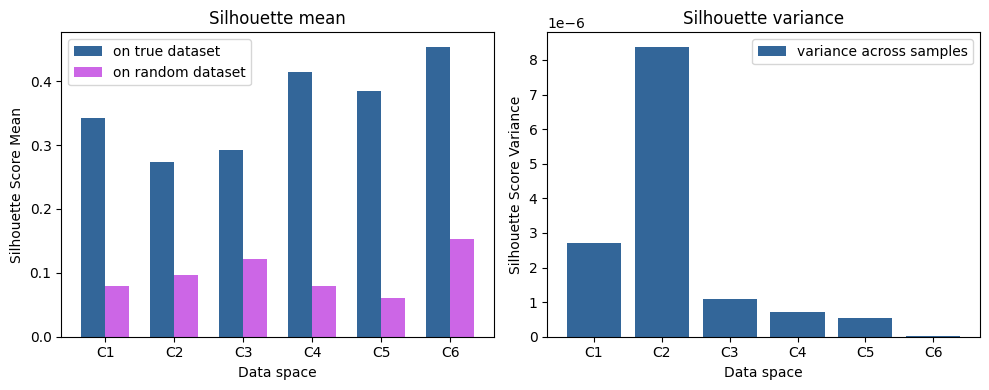
\includegraphics[width=.99\textwidth]{img/clustering/kmeans.png}
        \label{kmeans}
    \end{figure}
\end{frame}


%%%%%%%%%%%%%%%%%%%%%%%%%%%%%%%%%%%%%%%%%%%%%%%%%%%%%%%%%%%%%%%%%%%%%%%%%%

\begin{frame}{DBSCAN}

    \begin{exampleblock}{Selected features:}
        \begin{itemize}
            \item latitude
            \item min\_age\_participants
            \item n\_killed
        \end{itemize}
           
    \end{exampleblock}
    
    \begin{table}[]
        \centering
        \begin{tabular}{|lc|}
            \hline
              \textbf{Clustering}  & C4 \\
              $\epsilon$  & 0.6 \\
              $n$ & 21 \\
              \textbf{K} & 2\\
              \textbf{Clusters sizes} & (2088, 3938) \\
              \textbf{Silhouette} & 0.670266 \\
              \hline
        \end{tabular}
        \label{tab:my_label}
    \end{table}
\end{frame}

%%%%%%%%%%%%%%%%%%%%%%%%%%%%%%%%%%%%%%%%%%%%%%%%%%%%%%%%%%%%%%%%%%%%%%%%%%

\begin{frame}{DBSCAN}
    \begin{figure}
    \centering
    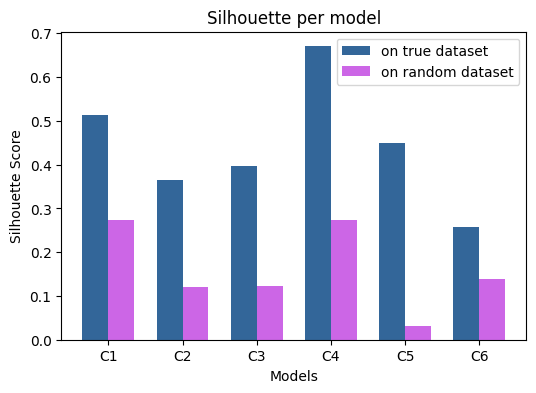
\includegraphics[width=.99\textwidth]{img/clustering/dbscan.png}
    \label{dbscan}
\end{figure}
\end{frame}

%%%%%%%%%%%%%%%%%%%%%%%%%%%%%%%%%%%%%%%%%%%%%%%%%%%%%%%%%%%%%%%%%%%%%%%%%%

\begin{frame}{Hierarchical Clustering}

    \begin{exampleblock}{Selected features:}
        \begin{itemize}
            \item latitude
            \item min\_age\_participants
            \item n\_killed
        \end{itemize}
    \end{exampleblock}

    
    
    \begin{table}[]
        \centering
        \begin{tabular}{|lc|}
            \hline  
            \textbf{Clustering}  & C4 \\
              \textbf{Best Method} & all\\
              \textbf{K} & 2\\
              \textbf{Clusters sizes} & (2088, 3938) \\
              \textbf{Silhouette} & 0.670266 \\
              \hline
        \end{tabular}
        \label{tab:my_label}
    \end{table}
\end{frame}

%%%%%%%%%%%%%%%%%%%%%%%%%%%%%%%%%%%%%%%%%%%%%%%%%%%%%%%%%%%%%%%%%%%%%%%%%%

\begin{frame}{Hierarchical Clustering}
    \begin{figure}
    \centering
    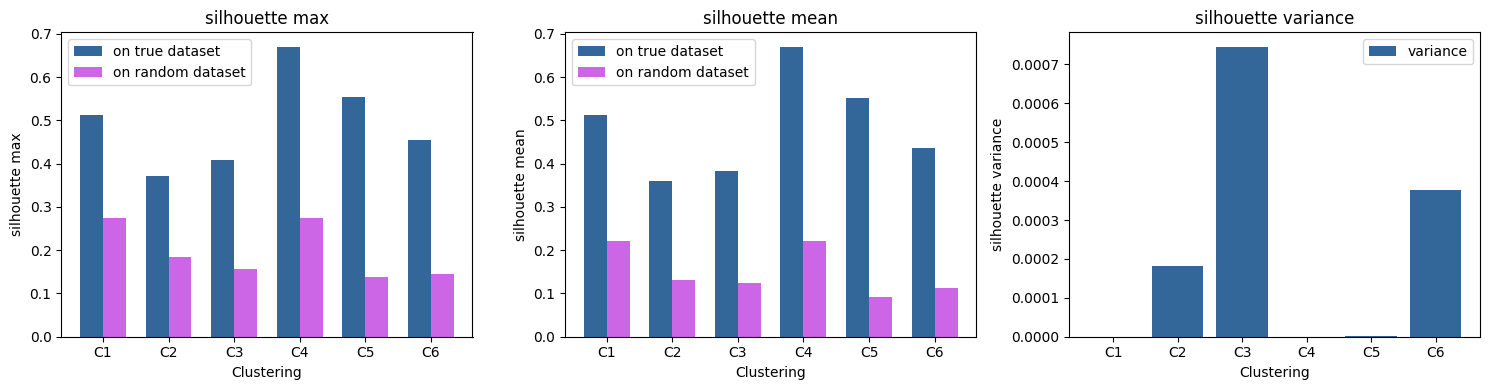
\includegraphics[width=.99\textwidth]{img/clustering/hier.png}
    \label{hier}
\end{figure}
\end{frame}

%%%%%%%%%%%%%%%%%%%%%%%%%%%%%%%%%%%%%%%%%%%%%%%%%%%%%%%%%%%%%%%%%%%%%%%%%%

\begin{frame}{DBSCAN and Hierarchical Clusters}
    \begin{figure}
    \centering
    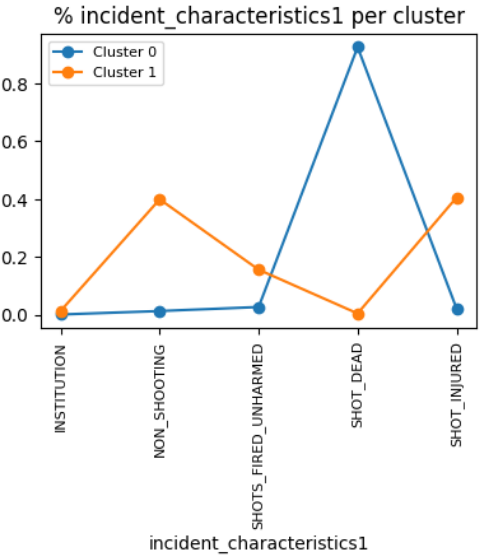
\includegraphics[scale=0.29]{img/clustering/dbscan1.png}
    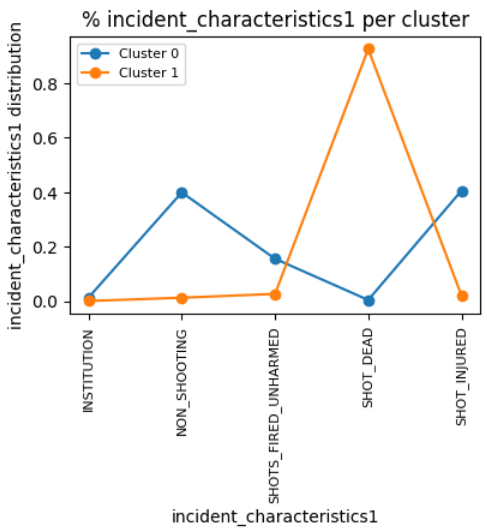
\includegraphics[scale=0.31]{img/clustering/hier2.png}
    \label{hier}
\end{figure}
\end{frame}